\begin{frame}
    \frametitle{Motores DC}
    \note{Información extraída de https://youtu.be/pEVsedl2KO4?si=_cwQpRPPUnQ04B3c}
    
    \begin{itemize}
        \item Imán Permanentemente estacionario
        \item Electromagnetismo induce torque
        \item Anillos divididos + brushes cambian la dirección de la corriente
    \end{itemize}
    
    \begin{figure}[!h]
        \subfloat[]{
            \movie[autostart,poster,loop,showcontrols]{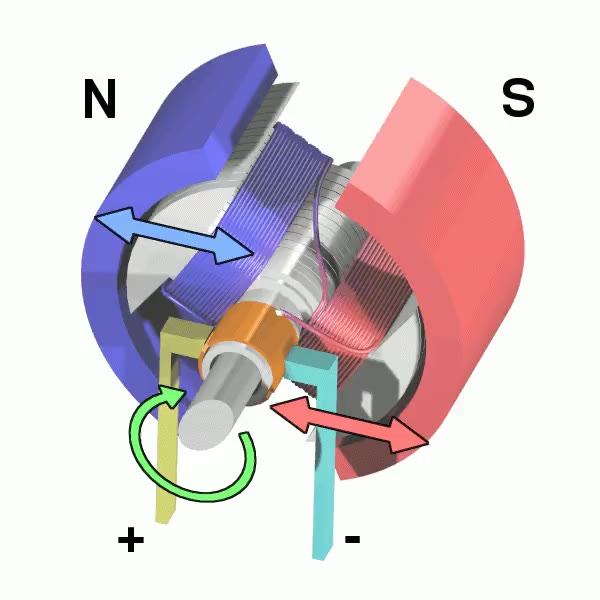
\includegraphics[width=0.2\columnwidth,valign=m]{images/dc_motor_3d_video.jpg}}{videos/dc_motor_3d.mp4}
        }
        \subfloat[]{
            \movie[autostart,poster,loop,showcontrols]{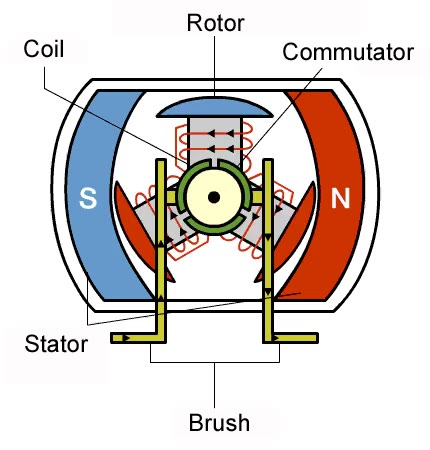
\includegraphics[width=0.2\columnwidth,valign=m]{images/dc_motor_video.jpg}}{videos/dc_motor.mp4}
        }
    \end{figure}
    
\end{frame}

\begin{frame}
    \frametitle{Controladores de Motores DC}
    \note{Información extraída de https://youtu.be/pEVsedl2KO4?si=_cwQpRPPUnQ04B3c}
    
    \begin{itemize}
        \item Más corriente = más rotación
        \item ¿Cómo modular corriente usando una señal digital?
        \item \emph{Pulse width modulation} (PWM)
        \item Duty cycle = ratio de tiempo vs periodo
    \end{itemize}
    
    \begin{figure}[!h]
        \subfloat[]{
            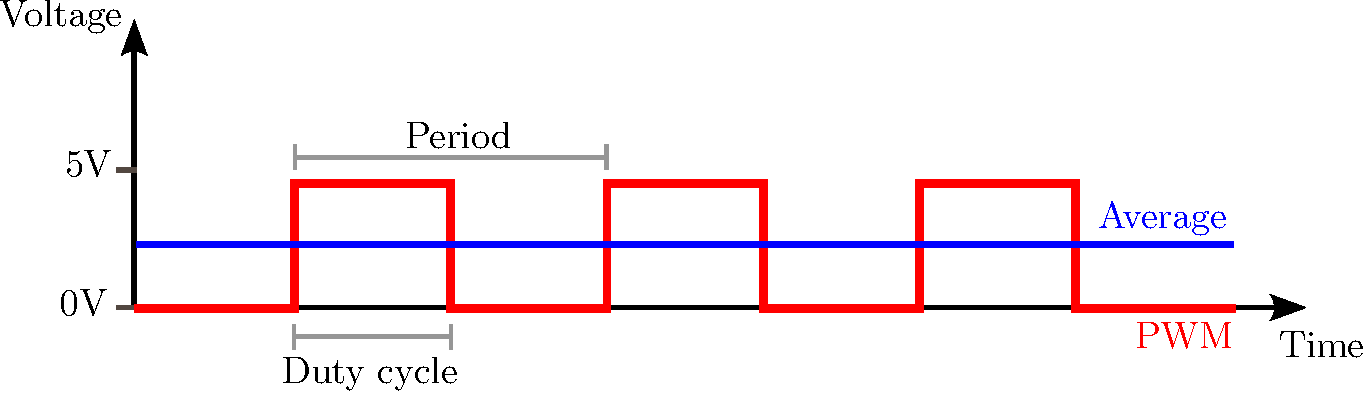
\includegraphics[width=0.6\columnwidth,valign=m]{images/pwm_signal.pdf}
        }
        \hfill
        \subfloat[]{
            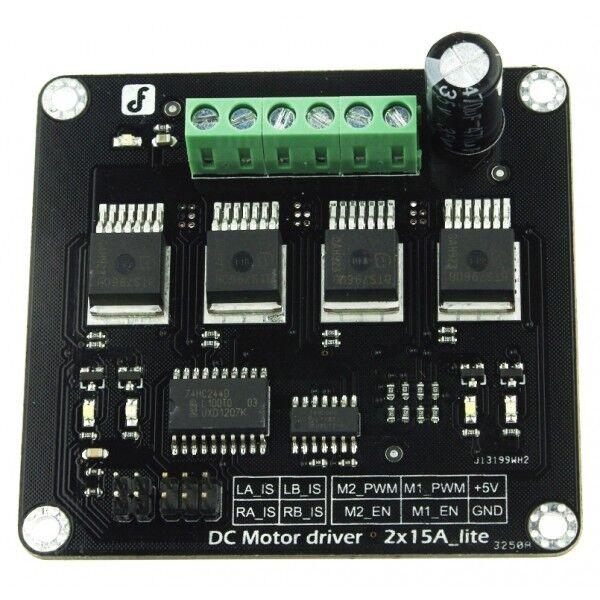
\includegraphics[width=0.3\columnwidth,valign=m]{images/dc_motor_driver_2x15A_lite.jpg}
        }
    \end{figure}
    
\end{frame}

\begin{frame}
    \frametitle{Open loop vs feedback control}
    \note{Información extraída de https://youtu.be/pEVsedl2KO4?si=_cwQpRPPUnQ04B3c}
    
    \begin{figure}[!h]
        \subfloat[Open loop control]{
            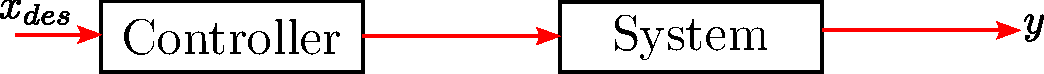
\includegraphics[width=0.6\columnwidth,valign=m]{images/open_loop_control.pdf}
        }
        
        \subfloat[Feedback control]{
            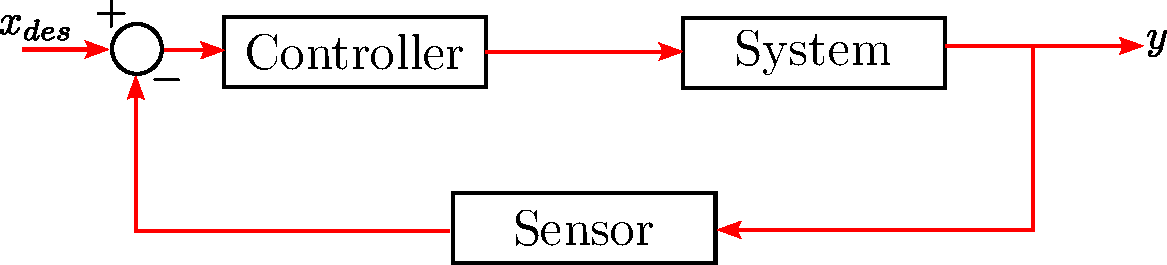
\includegraphics[width=0.7\columnwidth,valign=m]{images/feedback_control.pdf}
        }
    \end{figure}
    
\end{frame}

\begin{frame}
    \frametitle{Ejemplo de Feedback control}
    \note{Información extraída de https://youtu.be/pEVsedl2KO4?si=_cwQpRPPUnQ04B3c}
    
    \begin{center}
        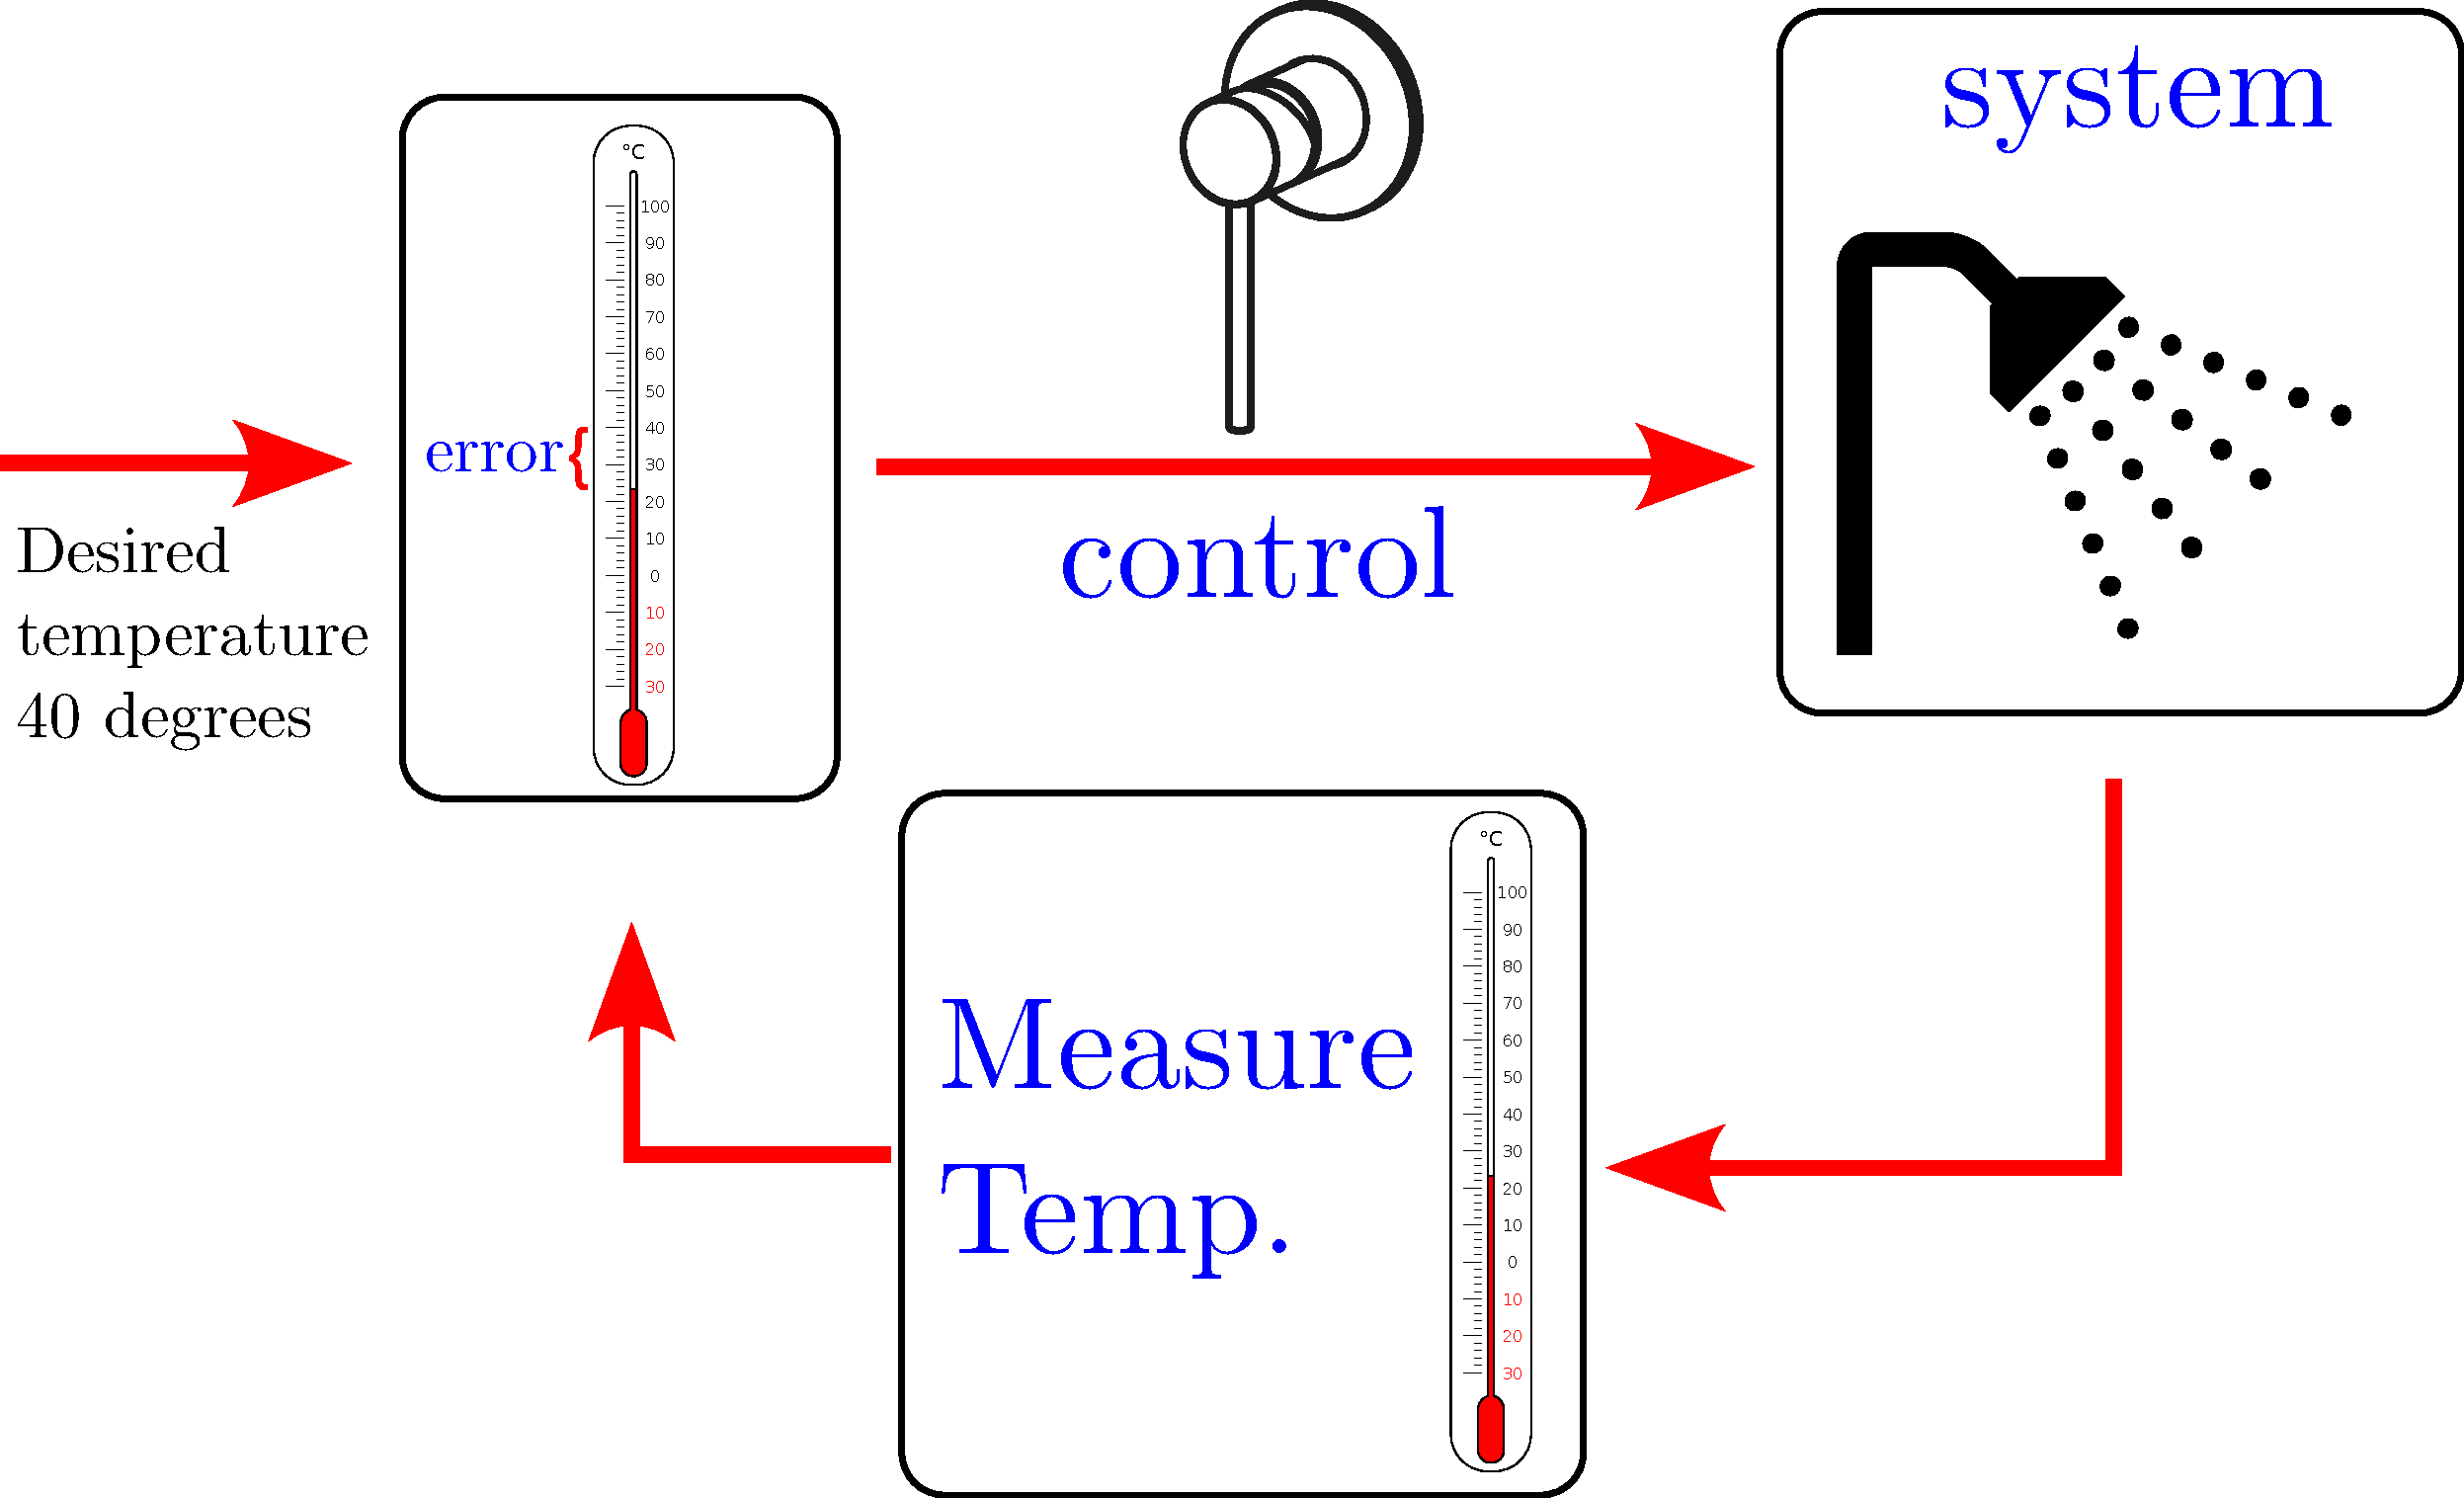
\includegraphics[width=0.6\columnwidth,valign=m]{images/temperature_feedback_control.pdf}
    \end{center}

    
\end{frame}

\begin{frame}
    \frametitle{Diagrama de bloques}
    \note{Información extraída de https://youtu.be/pEVsedl2KO4?si=_cwQpRPPUnQ04B3c}
    
    \begin{center}
        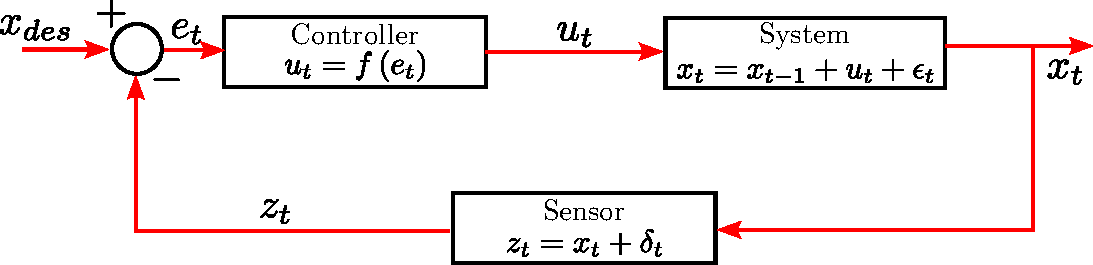
\includegraphics[width=0.8\columnwidth]{images/feedback_control_math.pdf}
    \end{center}
   
\end{frame}

\begin{frame}
    \frametitle{On-Off control}
    \note{Información extraída de https://youtu.be/pEVsedl2KO4?si=_cwQpRPPUnQ04B3c}
    
    \begin{center}
        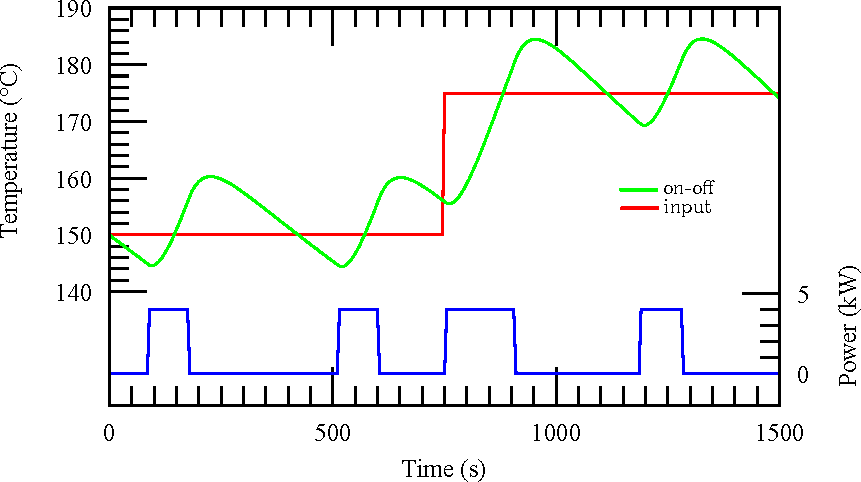
\includegraphics[width=0.8\columnwidth]{images/pid_control_on_off.pdf}
    \end{center}
    
    \note{Información extraída dehttps://www.zhinst.com/americas/de/resources/principles-of-pid-controllers}
    
    \note{Información extraída de https://newton.ex.ac.uk/teaching/CDHW/Feedback/ControlTypes.html}
    
\end{frame}

\begin{frame}
    \frametitle{Proportional control}
    \note{Información extraída de https://youtu.be/pEVsedl2KO4?si=_cwQpRPPUnQ04B3c}
    
    \begin{itemize}
        \item P-Control: $\controlCommand_{t} = K_{p} \error_{t}$ donde $\error_{t} = x_{des} - x_{t}$
    \end{itemize}
    
    \begin{center}
        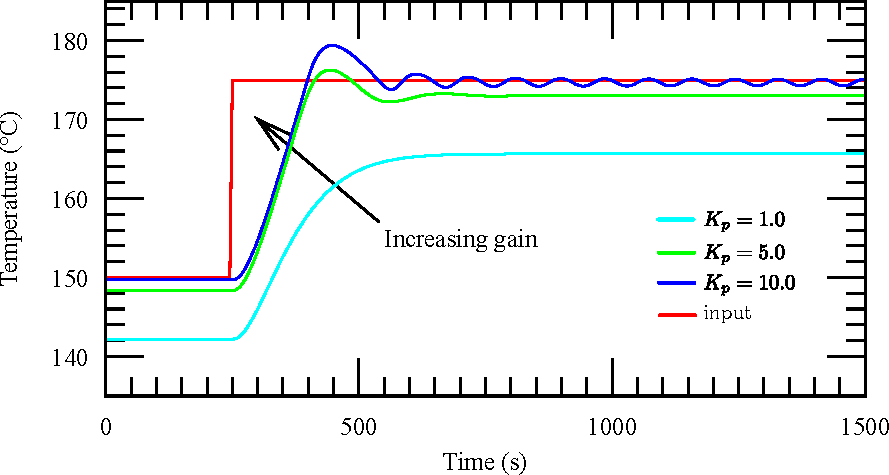
\includegraphics[width=0.8\columnwidth]{images/pid_control_proportional.pdf}
    \end{center}
    
    \note{Información extraída dehttps://www.zhinst.com/americas/de/resources/principles-of-pid-controllers}
    \note{Información extraída de https://newton.ex.ac.uk/teaching/CDHW/Feedback/ControlTypes.html}
    
\end{frame}

\begin{frame}
    \frametitle{Proportional+Derivative control}
    \note{Información extraída de https://youtu.be/pEVsedl2KO4?si=_cwQpRPPUnQ04B3c}
    
    \begin{itemize}
        \item PD-Control: $\controlCommand_{t} = K_{d} \error_{t}$
    \end{itemize}
    
    \begin{center}
        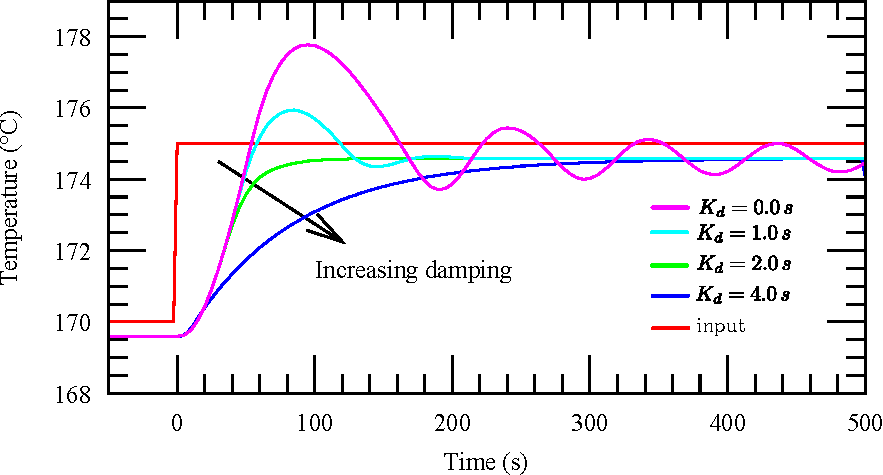
\includegraphics[width=0.8\columnwidth]{images/pid_control_derivative.pdf}
    \end{center}
    
    Un damping (amortiguación) demasiado pequeña produce overshoot y ringing, demasiado grande provoca una respuesta innecesariamente lenta.
    
    \note{Información extraída dehttps://www.zhinst.com/americas/de/resources/principles-of-pid-controllers}
    \note{Información extraída de https://newton.ex.ac.uk/teaching/CDHW/Feedback/ControlTypes.html}
    
    \note{Esta es la forma de control más sencilla y utilizada por casi todos los termostatos domésticos. Cuando el horno está más frío que la temperatura establecida, el calentador se enciende a la potencia máxima, M, y una vez que el horno está más caliente que la temperatura establecida, el calentador se apaga por completo. Las temperaturas de encendido y apagado se hacen deliberadamente para que difieran en una pequeña cantidad, conocida como histéresis H, para evitar que el ruido encienda el calentador rápidamente e innecesariamente cuando la temperatura está cerca del punto de ajuste. Las fluctuaciones de temperatura mostradas en el gráfico son significativamente mayores que la histéresis debido a la importante capacidad calorífica del elemento calefactor.}
\end{frame}

\begin{frame}
    \frametitle{Proportional+Integral+Derivative control}
    \note{Información extraída de https://youtu.be/pEVsedl2KO4?si=_cwQpRPPUnQ04B3c}
    
    \begin{itemize}
        \item PID-Control: $\controlCommand_{t} = K_{p} \error_{t}$
    \end{itemize}
    
    \begin{center}
        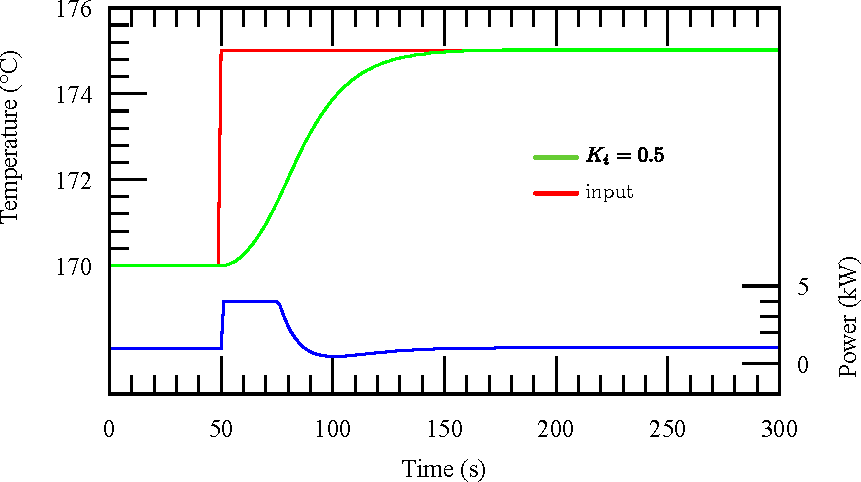
\includegraphics[width=0.8\columnwidth]{images/pid_control_integral.pdf}
    \end{center}
    
    \note{Información extraída dehttps://www.zhinst.com/americas/de/resources/principles-of-pid-controllers}
    \note{Información extraída de https://newton.ex.ac.uk/teaching/CDHW/Feedback/ControlTypes.html}
    
\end{frame}

\subsection{Position Control}

\begin{frame}
    \frametitle{Motivación: Position Control}
    \note{Información extraída de https://youtu.be/pEVsedl2KO4?si=_cwQpRPPUnQ04B3c}
    
    \begin{itemize}
        \item Mover el robot a una ubicación deseada $x_{des}$
        \item ¿Cómo generamos una señal de control adecuada $\controlCommand$?
        \item La localización del robot se estima mediante mediciones $\measurement$ de un sensor
    \end{itemize}
    
\end{frame}

\begin{frame}
    \frametitle{Cinemática de un cuerpo rígido}
    \note{Información extraída de https://youtu.be/pEVsedl2KO4?si=_cwQpRPPUnQ04B3c}
    
    \begin{itemize}
        \item Consideremos a un robot como un punto de masa
        \item Moviendo libremente en el espacio 1D
    \end{itemize}
    
\end{frame}

\begin{frame}
    \frametitle{Cinemática de un cuerpo rígido}
    \note{Información extraída de https://youtu.be/pEVsedl2KO4?si=_cwQpRPPUnQ04B3c}
    
    
    
    \TODO{Agregar imágenes }
    
\end{frame}


\begin{frame}
    \frametitle{P-control}
    \note{Información extraída de https://youtu.be/pEVsedl2KO4?si=_cwQpRPPUnQ04B3c}
    
    \begin{itemize}
        \item \TODO{Agregar imágenes }
    \end{itemize}
    
\end{frame}

\begin{frame}
    \frametitle{PD-control}
    \note{Información extraída de https://youtu.be/pEVsedl2KO4?si=_cwQpRPPUnQ04B3c}
    
    \begin{itemize}
        \item \TODO{Agregar imágenes }
    \end{itemize}
    
\end{frame}


\begin{frame}
\frametitle{PID-control}
\note{Información extraída de https://youtu.be/pEVsedl2KO4?si=_cwQpRPPUnQ04B3c}

\begin{itemize}
    \item \TODO{Agregar imágenes }
\end{itemize}

\end{frame}



\begin{frame}
    \frametitle{PID-control}
    \note{Información extraída de https://youtu.be/pEVsedl2KO4?si=_cwQpRPPUnQ04B3c}
    
    \begin{itemize}
        \item Estimar el error sistemático...
        \item PID-Control:
        \begin{equation*}
            \controlCommand_{t} = K_{p} \left(x_{des} - x_{t}\right) + K_{d} \left(\dot{x}_{des} - \dot{x}_{t} \right) + K_{i} \int_{0}^{t} \left( x_{des} - x_{t}\right) \, dt
        \end{equation*}
        
    \end{itemize}
    
    \begin{itemize}
        \item Funciona razonablemente para sistemas estables (con poco ruido)
        \item Puede ser peligroso en el caso en que se acumulen errores (\emph{wind-up effect})
    \end{itemize}
    
    \note{Si un robot se traba en un pozo y las ruedas siguen girando, la pose estimada por odometría y la verdadera localización del robot crece constantemente. El término integral del PID va a tomar valores enormes, ya que el error se acumula. En esta situación, si el robot se destrababa, vamos a tener una velocidad enorme y por lo tanto hacer que robot por ejemplo salte. Para esto el término integral puede únicamente tomar una ventana de tiempo (por ejemplo los últimos 5 segundos).}
    
    \note{El wind-up effect se refiere a cuando le damos un comando de control al robot pero los actuadores no son capaces de alcanzar el control solicitado. Esto puede ocasionar también que se acumule error.}
    
    
    \note{Información extraída dehttps://www.zhinst.com/americas/de/resources/principles-of-pid-controllers}
    \note{Información extraída de https://newton.ex.ac.uk/teaching/CDHW/Feedback/ControlTypes.html}
    
\end{frame}

\begin{frame}
    \frametitle{PID-control: Resumen}
    \note{Información extraída de https://youtu.be/pEVsedl2KO4?si=_cwQpRPPUnQ04B3c}
    
    \begin{itemize}
        \item P = control proportional, suficiente para la mayoría de los casos
        \item PD = reduce overshoot (por ejemplo, cuando la aceleración del vehículo puede ser controlada)
        \item PI = compensa errores o bias sistemáticos
        \item PID = combinación de todas las propiedades anteriores
    \end{itemize}
    
\end{frame}

\subsection{Trajectory control}

\begin{frame}
    \frametitle{Aplicación: Siguiendo una trayectoria}
    \note{Información extraída de https://youtu.be/pEVsedl2KO4?si=_cwQpRPPUnQ04B3c}
    
    \TODO{Agregar imagen}
    
\end{frame}

\begin{frame}
    \frametitle{Arquitectura de control}
    \note{Información extraída de https://youtu.be/pEVsedl2KO4?si=_cwQpRPPUnQ04B3c}
    
    \begin{center}
        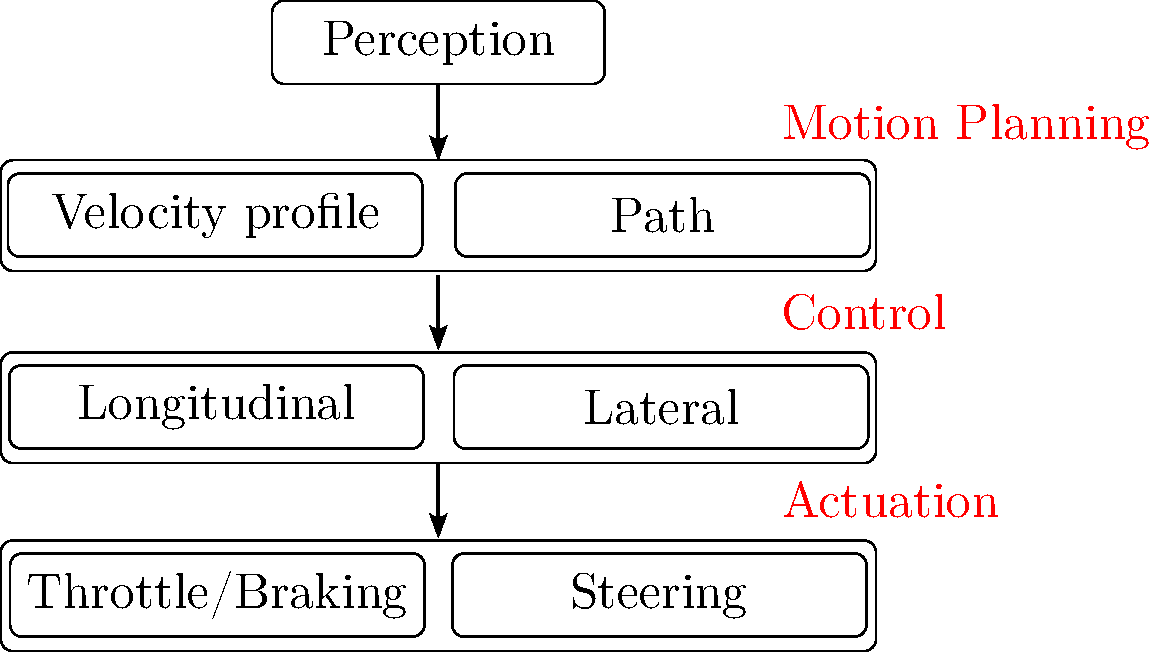
\includegraphics[width=0.8\columnwidth]{images/control_architecture2.pdf}
    \end{center}
    
     \note{Percepción: a través de los sensores armar un mapa del entorno}
     \note{Trayectoria = camino +perfil de velocidades. En cada pose del camino debemos saber con qué velocidad tenemos que llegar. Que cada punto de la trayectoria tenga un perfil de velocidad permite que el robot pueda moverse de manera suave de una pose a la otra.}
     \note{El control se divide en dos partes: longitudinal y lateral. El control Longitudinal hace referencia sobre la dirección de movimiento, es decir controlar la velocidad lineal. El control Lateral hace referencia que el robot este cerca del camino a seguir.}
\end{frame}

\begin{frame}
    \frametitle{Generación de trayectorias}
    \note{Información extraída de https://youtu.be/pEVsedl2KO4?si=_cwQpRPPUnQ04B3c}
    
    \begin{center}
        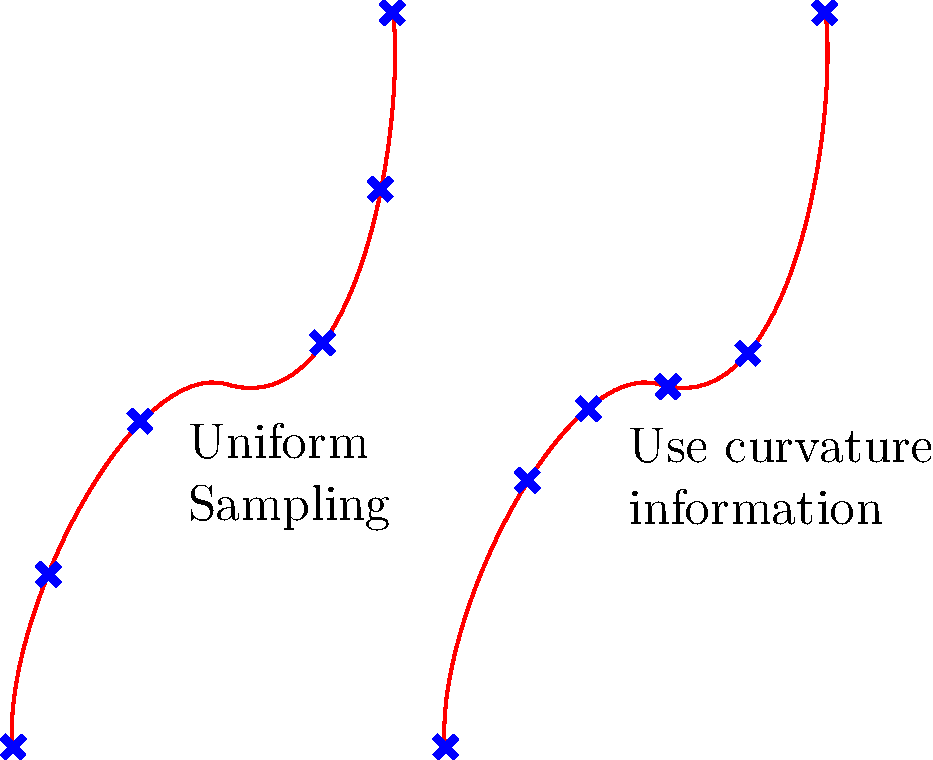
\includegraphics[width=0.6\columnwidth]{images/trajectory_generation.pdf}
    \end{center}
    
\end{frame}

\begin{frame}
    \frametitle{Ackermann Steering}
    \note{Información extraída de https://youtu.be/pEVsedl2KO4?si=_cwQpRPPUnQ04B3c}
    
    \begin{center}
        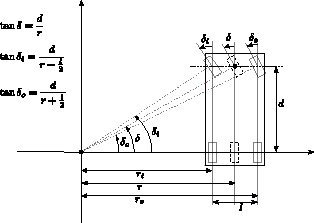
\includegraphics[width=0.6\columnwidth]{images/ackermann_steering.pdf}
    \end{center}
    
\end{frame}

\begin{frame}
    \frametitle{Ackermann Kinematics}
    \note{Información extraída de https://youtu.be/pEVsedl2KO4?si=_cwQpRPPUnQ04B3c}
    
    Estado: $\begin{bmatrix} x & y & \theta & \delta \end{bmatrix}^{\top}$ con $\delta = \tan^{-1}{\left(\frac{d}{r}\right)}$
    
    Control: $\begin{bmatrix} v & \dot{\delta} \end{bmatrix}^{\top}$
    
    
    \begin{center}
        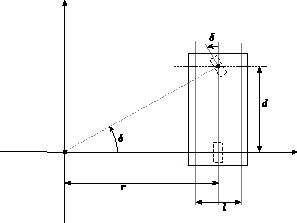
\includegraphics[width=0.6\columnwidth]{images/ackermann_kinematics.pdf}
    \end{center}
    
\end{frame}

\begin{frame}
    \frametitle{Control}
    \note{Información extraída de https://youtu.be/pEVsedl2KO4?si=_cwQpRPPUnQ04B3c}
    
    Restricciones:
    
    $v < v_{\max}$
    
    $v < |\delta_{\max}|$
    
    
    \begin{center}
        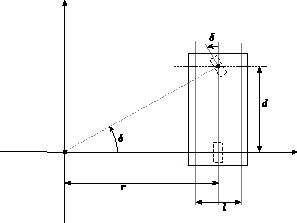
\includegraphics[width=0.6\columnwidth]{images/ackermann_kinematics.pdf}
    \end{center}
    
\end{frame}

\begin{frame}
    \frametitle{Longitudinal Control}
    \note{Información extraída de https://youtu.be/pEVsedl2KO4?si=_cwQpRPPUnQ04B3c}
        
    \begin{center}
        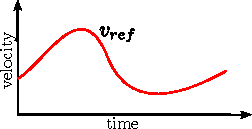
\includegraphics[width=0.6\columnwidth]{images/longitudinal_control.pdf}
    \end{center}
    
    \only<1->{¿Cómo podemos obtener esto?}
    \only<2->{Control PID}
    
\end{frame}


\begin{frame}
    \frametitle{Longitudinal Control}
    \note{Información extraída de https://youtu.be/pEVsedl2KO4?si=_cwQpRPPUnQ04B3c}
    
    \begin{center}
        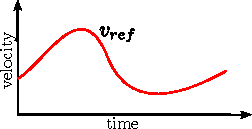
\includegraphics[width=0.6\columnwidth]{images/longitudinal_control.pdf}
    \end{center}
    
    \only<1->{¿Cómo podemos obtener esto?}
    \only<2->{Control PID}
    
\end{frame}

\begin{frame}
    \frametitle{Longitudinal Control}
    \note{Información extraída de https://youtu.be/pEVsedl2KO4?si=_cwQpRPPUnQ04B3c}
    
    \begin{center}
        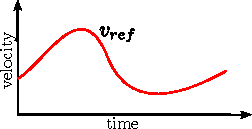
\includegraphics[width=0.6\columnwidth]{images/longitudinal_control.pdf}
    \end{center}
    
    \only<1->{¿Cómo podemos obtener esto?}
    \only<2->{Control PID}
    
\end{frame}


